\textbf{Ejemplo 2}\\
Un inversionista tiene dos opciones para invertir su dinero: en la primera opción, puede invertir 200.000 COP que le retornará 90.000 COP al final de cada año por los próximos 4 años, en la segunda opción, puede invertir hoy 300.000 COP y recibir 650.000 COP al final de 4 años. Si la tasa de interés es del 15\% nominal anual año vencido, determinar la mejor alternativa.
\\
\spanishdecimal{.}
\textbf{Solución.}\\
%La tabla ira centrada
\begin{center}
	\renewcommand{\arraystretch}{1.5}% Margenes de las celdas
	%Creación de la cuadricula de 3 columnas
\begin{longtable}[H]{|c|c|c|}
		%Creamos una linea horizontal
\hline
		%Definimos el color de la primera fila
\rowcolor[HTML]{FFB183}
		%%%%% INICIO ASIGNACIÓN PERÍODO FOCAL %%%%%%%
  %%%%%%%%%% INICIO TITULO
  %Lo que se hace aquí es mezclar las 3 columnas en una sola
  \multicolumn{3}{|c|}{\cellcolor[HTML]{FFB183}\textbf{1. Asignación período focal}}   \\ \hline
  %%%%%%%%%% FIN TITULO
  %%%%% INICIO DECLARACIÓN DE VARIABLES %%%%%%%
  \multicolumn{3}{|c|}{$pf : 0 pav$}   \\ \hline
  
%%%%%%%%%%% INICIO TITULO
\rowcolor[HTML]{FFB183}
\multicolumn{3}{|c|}{\cellcolor[HTML]{FFB183}\textbf{2. Declaración de variables}}    \\ \hline
%%%%%%%%%%% FIN TITULO
%%%%%%%%%%% INICIO MATEMÁTICAS        

\multicolumn{1}{|c|}{\cellcolor[HTML]{FFB183}\textbf{Valores monetarios}}    & \multicolumn{1}{c|}{\cellcolor[HTML]{FFB183}\textbf{Valores no monetarios}} & \multicolumn{1}{c|}{\cellcolor[HTML]{FFB183}\textbf{Incognitas}} \\ \hline

$ P_1 = 200.000COP $	& $ j=15\% naav $ &	{$B/C_1=?$} \\
$ P_2 = 300.000COP $	& $ i = 15\% pav $ &{$B/C_2=?$} \\
$\quad \quad \quad \quad \quad  R_{1} = 90.000 COP \quad \quad \quad \quad \quad  $ & &{$ VP_1= ? COP $} \\
$ R_{2} =  650.000 COP $	&& {$VP_2= ? COP$} \\
	&&	{$VPN_1=?$} \\
$  $	                        &&	{$VPN_2=?$} \\

\hline
%%%%%%%%%% FIN MATEMÁTICAS
		%%%%% INICIO FLUJO DE CAJA
\rowcolor[HTML]{FFB183}
\multicolumn{3}{|c|}{\cellcolor[HTML]{FFB183}\textbf{3. Diagrama de flujo de caja}} \\ \hline
		%Mezclamos 3 columnas y pondremos el dibujo
		%%%%%%%%%%%%% INSERCIÓN DE LA IMAGEN
		%Deberán descargar las imágenes respectivas del drive y pegarlas en la carpeta
		%n_capitulo/img/ejemplos/1/capitulo1ejemplo1.pdf  (el /1/ es el numero del ejemplo)
\multicolumn{3}{|c|}{ 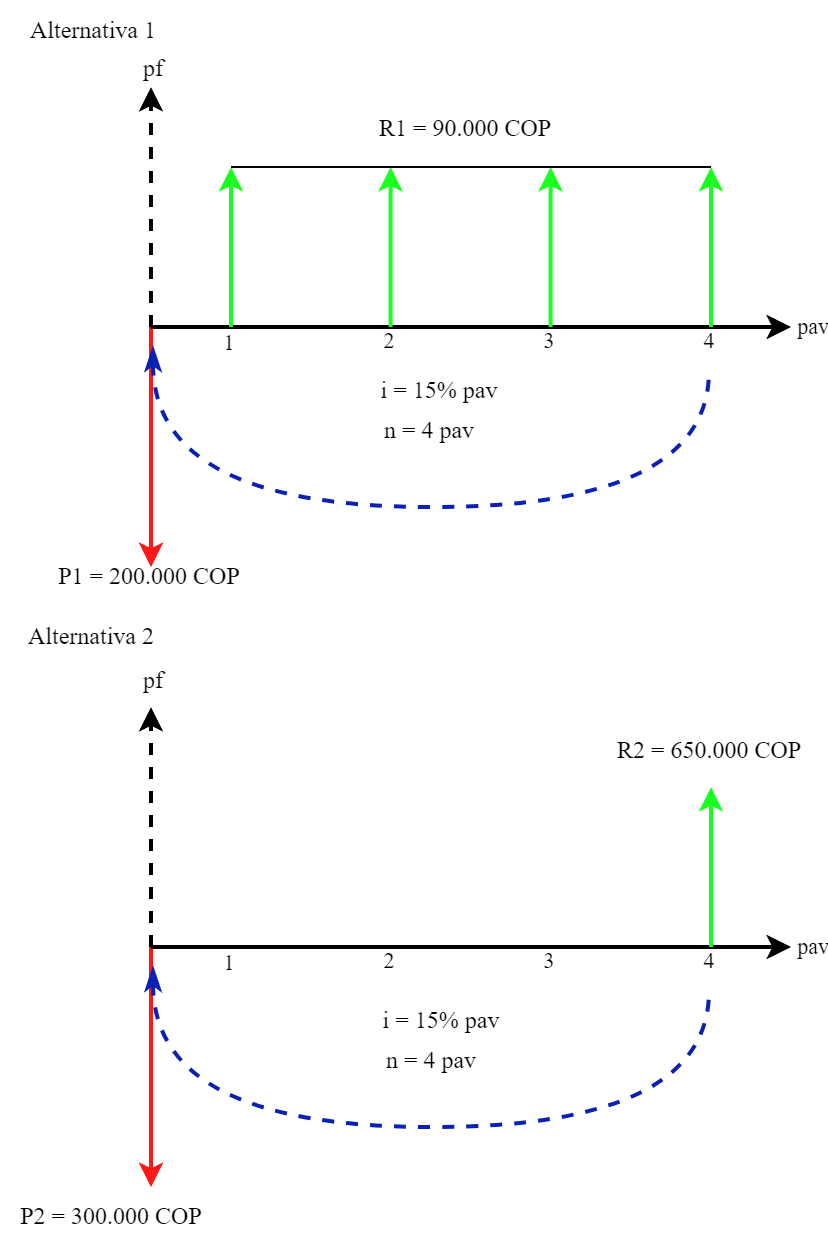
\includegraphics[width=10.5cm]{EJ2_1.png}} 

   \\\hline
		%%%%%%%%%%%%% FIN INSERCIÓN DE IMAGEN
		%%%%%FIN FLUJO DE CAJA
		
		
		
		%%%%% INICIO DECLARACIÓN FORMULAS
		%%%%%%%%%%% INICIO TITULO
\rowcolor[HTML]{FFB183}
\multicolumn{3}{|c|}{\cellcolor[HTML]{FFB183}\textbf{4. Declaración de fórmulas}}    \\ \hline
%%%%%%%%%%% FIN TITULO
%%%%%%%%%%% INICIO MATEMÁTICAS
\multicolumn{3}{|c|} {$ \quad \quad \quad \quad \quad \quad \quad VPN = \Sigma(Ingresos) - \Sigma(Inversiones) $\hspace{15pt}\textit{Valor Presente Neto \quad \quad \quad \quad \quad \quad \quad}}   \\ 
\multicolumn{3}{|c|} {$VP = R\frac{1-(1+i)^{-n}}{i}$\hspace{15pt}\textit{Valor Presente Serie Uniforme Vencida}}   \\ 
\multicolumn{3}{|c|} {$P = F(1+i)^{-n}$\hspace{15pt}\textit{Valor Presente}}   \\ 
\multicolumn{3}{|c|} {$B/C = \frac{VPI}{VPC}$\hspace{15pt}\textit{ Relación Beneficio/Costo}}   \\ 
\hline	
	
		%%%%%%%%%% FIN MATEMÁTICAS
		%%%%%% INICIO DESARROLLO MATEMÁTICO
\rowcolor[HTML]{FFB183}
		%%%%%%%%%%INICIO TITULO
\multicolumn{3}{|c|}{\cellcolor[HTML]{FFB183}\textbf{5. Desarrollo matemático Opcion 1}}       \\ \hline
		%%%%%%%%%% FIN TITULO
		%%%%%%%%%% INICIO MATEMÁTICAS
        \multicolumn{3}{|c|}{$ VP_1 = 90.000 COP \frac{1-(1 + 0.15)^{-4}}{0.15} = 256.948,052 COP $}  
		\\
		\multicolumn{3}{|c|}{$ B/C_1 = \frac{256.948,052 COP}{200.000 COP} = 1,28 $}
        \\
		\multicolumn{3}{|c|}{$ B/C_1 = 1,28 > 1 $}  
		\\
		\multicolumn{3}{|c|}{$ VPN_1 = 256.948,052 COP -200.000 COP = 56.948 COP $}  
		\\
	    \hline
				
		%%%%%%%%%% FIN MATEMÁTICAS
		%%%%%% FIN DESARROLLO MATEMÁTICO

		%%%%%% INICIO DESARROLLO MATEMÁTICO
\rowcolor[HTML]{FFB183}
		%%%%%%%%%%INICIO TITULO
\multicolumn{3}{|c|}{\cellcolor[HTML]{FFB183}\textbf{6. Desarrollo matemático Opcion 2}}       \\ \hline
		%%%%%%%%%% FIN TITULO
		%%%%%%%%%% INICIO MATEMÁTICAS
        \multicolumn{3}{|c|}{$ VP_2 = 650.000 COP \frac{(1+0.15)^{-4}}{0.15} = 371.639,6 COP $}  
		\\
		\multicolumn{3}{|c|}{$ B/C_2 = \frac{371.639,6 COP COP}{300.000 COP} = 1,24 $}
        \\
		\multicolumn{3}{|c|}{$ B/C_2 = 1,24 > 1 $}  
		\\
		\multicolumn{3}{|c|}{$ VPN_2 = 371.639,6 COP -300.000 COP = 71.640 COP $}  
		\\
	    \hline
				
		%%%%%%%%%% FIN MATEMÁTICAS
		%%%%%% FIN DESARROLLO MATEMÁTICO


		%%%%%% INICIO RESPUESTA
\rowcolor[HTML]{FFB183}
		%%%%%%%%%%INICIO TITULO
\multicolumn{3}{|c|}{\cellcolor[HTML]{FFB183}\textbf{7. Respuesta}}   \\ \hline
		%%%%%%%%%% FIN TITULO
		%%%%%%%%%% INICIO RESPUESTA MATEMÁTICA
		
\multicolumn{3}{|c|}{ \text{Se evidencia una contradicción, ya que al calcular el beneficio costo de cada opcion, se tiene que} } \\ 
\multicolumn{3}{|c|}{ \text{la mejor es la primera. Sin embargo, al comparar con el VPN la mejor es la segunda.} } \\ 
\hline
		
		
		%%%%%%%%%% FIN MATEMÁTICAS
		%%%%%% FIN RESPUESTA
	\end{longtable}
	%Se crean dos lineas en blanco para que no quede el siguiente texto tan pegado
	%\newline \newline %USARLO SI CREES QUE ES NECESARIO
\end{center}


%Tabla 2
%La tabla ira centrada
\begin{center}
	\renewcommand{\arraystretch}{1.5}% Margenes de las celdas
	%Creación de la cuadricula de 3 columnas
\begin{longtable}[H]{|c|c|c|}
		%Creamos una linea horizontal
\hline
		%Definimos el color de la primera fila
\rowcolor[HTML]{FFB183}
		%%%%% INICIO ASIGNACIÓN PERÍODO FOCAL %%%%%%%
  %%%%%%%%%% INICIO TITULO
  %Lo que se hace aquí es mezclar las 3 columnas en una sola
  \multicolumn{3}{|c|}{\cellcolor[HTML]{FFB183}\textbf{1. Asignación período focal}}   \\ \hline
  %%%%%%%%%% FIN TITULO
  %%%%% INICIO DECLARACIÓN DE VARIABLES %%%%%%%
  \multicolumn{3}{|c|}{$pf : 0 pav$}   \\ \hline
  
%%%%%%%%%%% INICIO TITULO
\rowcolor[HTML]{FFB183}
\multicolumn{3}{|c|}{\cellcolor[HTML]{FFB183}\textbf{2. Declaración de variables}}    \\ \hline
%%%%%%%%%%% FIN TITULO
%%%%%%%%%%% INICIO MATEMÁTICAS

\multicolumn{1}{|c|}{\cellcolor[HTML]{FFB183}\textbf{Valores monetarios}}    & \multicolumn{1}{c|}{\cellcolor[HTML]{FFB183}\textbf{Valores no monetarios}} & \multicolumn{1}{c|}{\cellcolor[HTML]{FFB183}\textbf{Incognitas}} \\ \hline

$ P_1 = 200.000COP $	& $ j=15\% naav $ & \\
$ P_2 = 300.000COP $	& $ i = 15\% pav $ &{$B/C=?$} \\
$\quad \quad \quad \quad \quad  R_{1} = 90.000 COP \quad \quad \quad \quad \quad  $ &&  \\
$ R_{2} =  650.000 COP $	&& {$R_{b-a} = ?$} \\

\hline
%%%%%%%%%% FIN MATEMÁTICAS
		%%%%% INICIO FLUJO DE CAJA

\rowcolor[HTML]{FFB183}
\multicolumn{3}{|c|}{\cellcolor[HTML]{FFB183}\textbf{3. Tabla método incremental}} \\ \hline
		%Mezclamos 3 columnas y pondremos el dibujo
		%%%%%%%%%%%%% INSERCIÓN DE LA IMAGEN
		%Deberán descargar las imágenes respectivas del drive y pegarlas en la carpeta
		%n_capitulo/img/ejemplos/1/capitulo1ejemplo1.pdf  (el /1/ es el numero del ejemplo)

\multicolumn{3}{|c|}{}    \\
\multicolumn{3}{|c|}{
    \begin{tabular}{|c|c|c|c|}
        \hline
            \cellcolor[HTML]{FFB183}Año & \cellcolor[HTML]{FFB183}A            & \cellcolor[HTML]{FFB183}B            & \cellcolor[HTML]{FFB183}{B - A}        \\ \hline
            0   & -200.000 COP & -300.000 COP & -100.000 COP \\ \hline
            1   & 90.000 COP   & 0 COP        & -90.000 COP  \\ \hline
            2   & 90.000 COP   & 0 COP        & -90.000 COP  \\ \hline
            3   & 90.000 COP   & 0 COP        & -90.000 COP  \\ \hline
            4   & 90.000 COP   & 650.000 COP  & 560.000 COP  \\ \hline
    \end{tabular}
} \\
\multicolumn{3}{|c|}{}  \\ \hline
		%%%%%%%%%%%%% FIN INSERCIÓN DE IMAGEN
		%%%%%FIN FLUJO DE CAJA

\rowcolor[HTML]{FFB183}
\multicolumn{3}{|c|}{\cellcolor[HTML]{FFB183}\textbf{4. Diagrama de flujo de caja}} \\ \hline
		%Mezclamos 3 columnas y pondremos el dibujo
		%%%%%%%%%%%%% INSERCIÓN DE LA IMAGEN
		%Deberán descargar las imágenes respectivas del drive y pegarlas en la carpeta
		%n_capitulo/img/ejemplos/1/capitulo1ejemplo1.pdf  (el /1/ es el numero del ejemplo)
\multicolumn{3}{|c|}{ 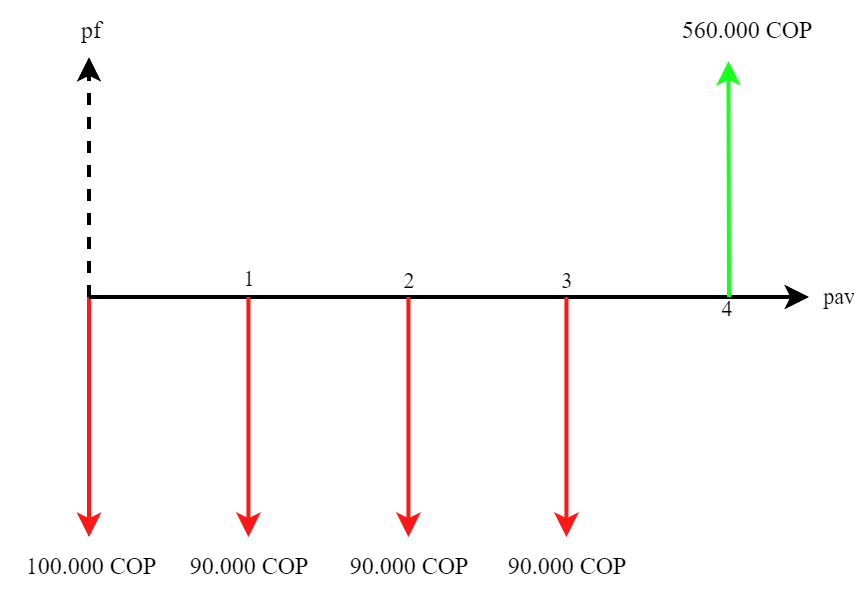
\includegraphics[width=10.5cm]{EJ2_2.png}}
   \\\hline
		%%%%%%%%%%%%% FIN INSERCIÓN DE IMAGEN
		%%%%%FIN FLUJO DE CAJA
		
		
		%%%%% INICIO DECLARACIÓN FORMULAS
		%%%%%%%%%%% INICIO TITULO
\rowcolor[HTML]{FFB183}
\multicolumn{3}{|c|}{\cellcolor[HTML]{FFB183}\textbf{5. Declaración de fórmulas}}    \\ \hline
%%%%%%%%%%% FIN TITULO
%%%%%%%%%%% INICIO MATEMÁTICAS
\multicolumn{3}{|c|} {$ \quad \quad \quad \quad \quad \quad \quad \quad \quad B/C = \frac{VPI}{VPC}$\hspace{15pt}\textit{Relación Beneficio/Costo \quad \quad \quad \quad \quad \quad \quad \quad \quad}}   \\ 
\multicolumn{3}{|c|} {$VP = R\frac{1-(1+i)^{-n}}{i}$\hspace{15pt}\textit{Valor Presente Serie Uniforme Vencida}}   \\
\hline	
	
		%%%%%%%%%% FIN MATEMÁTICAS
		%%%%%% INICIO DESARROLLO MATEMÁTICO
\rowcolor[HTML]{FFB183}
		%%%%%%%%%%INICIO TITULO
\multicolumn{3}{|c|}{\cellcolor[HTML]{FFB183}\textbf{6. Desarrollo matemático Opcion 1}}       \\ \hline
		%%%%%%%%%% FIN TITULO
		%%%%%%%%%% INICIO MATEMÁTICAS
        \multicolumn{3}{|c|}{$B/C = \frac{560.000COP(1+0.15)^{-4}}{100.000COP + 90.000COP\frac{1-(1+0.15)^{-3}}{0.15}} = 1,048 > 1$}  
		\\
	    \hline
				
		%%%%%%%%%% FIN MATEMÁTICAS
		%%%%%% FIN DESARROLLO MATEMÁTICO


		%%%%%% INICIO RESPUESTA
\rowcolor[HTML]{FFB183}
		%%%%%%%%%%INICIO TITULO
\multicolumn{3}{|c|}{\cellcolor[HTML]{FFB183}\textbf{7. Respuesta}}   \\ \hline
		%%%%%%%%%% FIN TITULO
		%%%%%%%%%% INICIO RESPUESTA MATEMÁTICA

\multicolumn{3}{|c|}{ \text{Esto significa que sí se puede aceptar el exceso de inversión, lo cual corrobora la decisión tomada}} \\ 
\multicolumn{3}{|c|}{ \text{mediante el VPN en el sentido de señalar la segunda opción como la mejor.}} \\ 
\hline
		
		
		%%%%%%%%%% FIN MATEMÁTICAS
		%%%%%% FIN RESPUESTA
	\end{longtable}
	%Se crean dos lineas en blanco para que no quede el siguiente texto tan pegado
	%\newline \newline %USARLO SI CREES QUE ES NECESARIO
\end{center}
%%%%%%%%%%%%%%%%%%%%%%%%%%FIN EJERCICIO 1 %%%%%%%%%%%%%%%%%%%%%%%%%%%
